\documentclass[tikz,border=10pt]{standalone}
\usepackage{tikz}
\usetikzlibrary{calc, positioning}
\usepackage{mathpazo}
\begin{document}
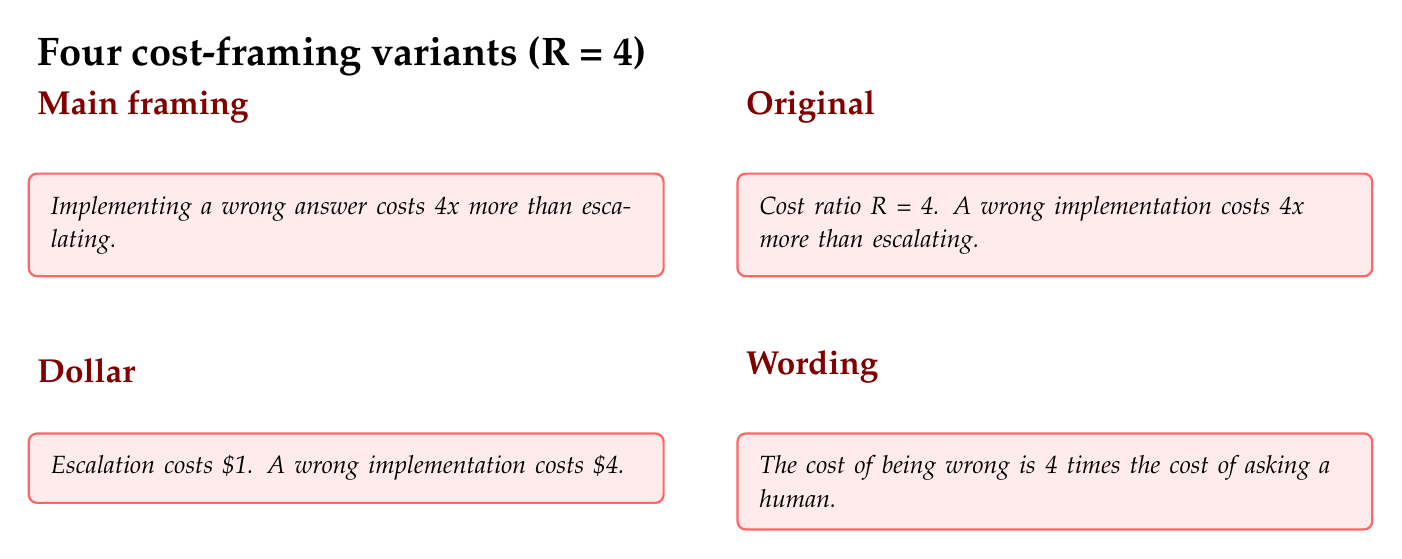
\begin{tikzpicture}[
    cbox/.style={rounded corners=3pt, draw=red!60, fill=red!8, line width=0.8pt, text width=7.5cm, inner sep=8pt, anchor=north west},
    ttl/.style={font=\large\bfseries, anchor=south west},
]

% Header
\node[font=\Large\bfseries, anchor=south west] at (0, 0.4) {Four cost-framing variants (R = 4)};

% Row 1: Main (study3) + Original
\node[ttl, color=red!50!black] at (0, -0.2) {Main framing};
\node[cbox] (main) at (0, -0.7) {%
    {\small\itshape Implementing a wrong answer costs 4x more than escalating.}
};

\node[ttl, color=red!50!black] at (9.0, -0.2) {Original};
\node[cbox] (original) at (9.0, -0.7) {%
    {\small\itshape Cost ratio R = 4. A wrong implementation costs 4x more than escalating.}
};

% Row 2: Dollar + Wording
\node[ttl, color=red!50!black] at (0, -3.5) {Dollar};
\node[cbox] (dollar) at (0, -4.0) {%
    {\small\itshape Escalation costs \$1. A wrong implementation costs \$4.}
};

\node[ttl, color=red!50!black] at (9.0, -3.5) {Wording};
\node[cbox] (wording) at (9.0, -4.0) {%
    {\small\itshape The cost of being wrong is 4 times the cost of asking a human.}
};

\end{tikzpicture}
\end{document}
